\section{Features and Implementation}

\mkado is implemented in Python
and provides both a command-line interface built on
\texttt{Typer} and a Python API for programmatic use.
It accepts codon-aligned FASTA files as input,
requiring no pre-processing or external format conversion.
Sequences are automatically partitioned into ingroup and outgroup sets
by name pattern matching,
supporting both multi-species alignments in a single FASTA file
and separate files containing ingroup or outgroup sequences.
\revpoint{1}{1}\revpoint{2}{2}\mkado{} also accepts variant-call
input via the \texttt{vcf} subcommand, which takes a multi-sample
ingroup VCF, a single-sample outgroup VCF, a reference FASTA, and a
GFF3 annotation, derives codon-level polymorphism and divergence
counts directly, and supports the full set of MK analyses available
to the FASTA workflow. Together, these two input modes distinguish
\mkado{} from FASTA-only tools (\texttt{DnaSP}, \texttt{asymptoticMK})
and from VCF-only tools (\texttt{degenotate}, \texttt{fastDFE}).
Full documentation, including tutorials and API reference,
is available at \url{https://mkado.readthedocs.io}.

\paragraph{Analysis methods}
\mkado implements five MK-based analyses.
The \textit{standard} test computes the classical $2 \times 2$ table
of nonsynonymous and synonymous changes
in polymorphism and divergence,
with significance assessed by Fisher's exact test
or the $G$-test.
\revpoint{2}{1}$D_n$ and $D_s$ are the numbers of fixed differences
between ingroup and outgroup at codon positions where the inferred
substitution is nonsynonymous or synonymous, respectively, under the
supplied genetic code.
$P_n$ and $P_s$ are the corresponding numbers of ingroup
polymorphic sites at which the derived (non-outgroup) allele
segregates above an optional frequency threshold
(default zero, i.e.\ all polymorphisms;
\texttt{-{}-min-freq~$X$} excludes sites with derived allele
frequency below $X$, and \texttt{-{}-no-singletons} excludes
singletons by setting the threshold to $1/n$ for sample size $n$).
By default $P_n$ and $P_s$ follow the \texttt{DnaSP} convention
and exclude sites that also segregate in the outgroup;
\texttt{-{}-pool-polymorphisms} pools ingroup and outgroup
polymorphism instead.
Summary statistics include the neutrality index \citep[NI;][]{rand1996},
$\alpha$ \citep{smith2002},
and the Direction of Selection statistic
\citep[DoS;][]{stoletzki2011}.
\revpoint{1}{2}Tests that depend on derived allele frequency---the
asymptotic and imputed MK tests described below---require knowing the
derived allele at each polymorphic site. \mkado{} polarizes alleles
automatically using the outgroup: at each polymorphic site, the
allele matching the outgroup is treated as ancestral and any
non-outgroup allele as derived. This automatic single-outgroup
polarization is distinct from the \textit{polarized} MK test below,
which uses a \emph{second} outgroup to attribute each fixed
difference to either the ingroup or the outgroup lineage.
The \textit{polarized} test uses a second outgroup
to infer the ancestral state at each fixed difference,
assigning divergence to the ingroup or outgroup lineage
for lineage-specific inference.
The \textit{asymptotic} test bins polymorphisms
by derived allele frequency,
computes $\alpha$ within each bin,
and fits an exponential model $\alpha(x) = a + b e^{-cx}$
to extrapolate the asymptotic $\alpha$ at $x = 1$,
correcting for the contribution of weakly deleterious variants
\citep{messer2013}.
A linear model is also fitted
and AIC selects the better specification,
following \citet{haller2017}.
\revpoint{1}{4}\mkado{} supports both the original per-bin SFS construction of
\citet{messer2013}, in which $P_n(x)$ and $P_s(x)$ count
polymorphic sites with derived allele frequency \emph{equal to}~$x$,
and the cumulative inclusive variant of \citet{uricchio2019}, in
which $P_n(x)$ and $P_s(x)$ count polymorphic sites with derived
allele frequency \emph{at or above}~$x$ (selectable with
\texttt{-{}-sfs-mode \{at,above\}}); the cumulative form has the
same asymptote at $x = 1$ but is more robust to bin-count sparsity
in large samples.
The asymptotic test supports both per-gene
and aggregated (pooled across genes) modes; for the aggregated
mode, two confidence-interval methods are available
(\texttt{-{}-ci-method}): a parametric Monte-Carlo procedure that
samples the curve-fit covariance matrix (default; fast) and a
case-resampling bootstrap that resamples the pooled polymorphism
list and refits per replicate (slower per replicate but more
principled when per-bin counts are small).
The \textit{imputed} test corrects for weakly deleterious mutations
by estimating their contribution from the ratio
of low- to high-frequency synonymous polymorphisms
\citep{murga-moreno2022}.
Polymorphisms are split at a derived allele frequency % Alternatively, change to DAF here
cutoff (default 15\%),
and the expected number of weakly deleterious nonsynonymous
polymorphisms below the cutoff is imputed as
$P_{wd} = P_{n,\text{low}} - P_{n,\text{high}} \times
(P_{s,\text{low}} / P_{s,\text{high}})$.
The corrected count $P_{n}^{*} = P_n - P_{wd}$
is then used in the standard $2 \times 2$ test
to obtain a bias-corrected $\alpha$.
This approach retains more data than simple frequency filtering
while still removing the downward bias from slightly deleterious
variants.
Finally, the Tarone-Greenland $\alpha_\text{TG}$ estimator
\citep{stoletzki2011}
provides an unbiased multi-gene estimate of $\alpha$
by weighting each gene inversely by $P_s + D_s$,
correcting for sample size heterogeneity across loci.

\paragraph{Codon change classification}
When comparing codons that differ at multiple positions,
the assignment of changes as synonymous or nonsynonymous
is not straightforward
because the order of substitutions is unknown.
\mkado pre-computes all shortest mutational paths
between every pair of codons
and weights the synonymous and nonsynonymous contributions
equally across paths,
following the approach of \citet{nei1986}.

\paragraph{Batch processing and output}
MKado's \texttt{batch} command processes directories of alignment files
in parallel using Python's multiprocessing facilities
with configurable worker counts.
Benjamini-Hochberg false discovery rate (FDR) $q$-values
are computed automatically across all genes.
Results are available in human-readable, TSV, or JSON formats.
A companion \texttt{info} command reports alignment diagnostics
(sequence count, length, and codon structure)
for input validation.

To evaluate scaling performance,
we benchmarked \mkado on 12,437 human protein-coding genes
aligned with chimpanzee and orangutan orthologs
from \texttt{OrthoMaM} \citep{orthomam2024},
with polymorphism data from 178 Yoruba individuals
in the 1000 Genomes Project \citep{1000genomes2015}.
Processing all genes with 128 worker threads
completed in 28 seconds, a $\sim$50$\times$ speedup over
single-threaded execution.\revpoint{2}{10} Per-gene work
(alignment parsing, codon classification, and the per-gene MK
computation) takes only milliseconds, so the per-process spawn
overhead from Python's \texttt{multiprocessing} grows
non-negligible relative to per-task work as the worker count
rises. \Cref{fig:benchmark} shows approximately linear scaling
up to roughly 16 workers, with progressively diminishing
efficiency past 32 workers; we therefore recommend setting the
worker count well below the gene count for batch runs at any
scale. For workloads dominated by aggregated tests (asymptotic
MK with case-resampling bootstrap CIs), where per-task work is
much larger, scaling extends usefully to higher worker counts
(\cref{fig:aggregated_runtime}).

\paragraph{Visualization}
\mkado generates publication-ready plots
directly from the command line.
Volcano plots display $-\log_{10}(\text{NI})$
against $-\log_{10}(p)$ for each gene,
with Bonferroni and nominal significance thresholds
(left panel of \cref{fig:volcano}).
The asymptotic test produces $\alpha(x)$ curves
showing the fitted model and bootstrap confidence intervals
(right panel of \cref{fig:volcano}).

\begin{figure*}[!t]
  \centering
  \includegraphics[width=0.48\textwidth]{figures/mk_volcano_pongo.png}\hfill
  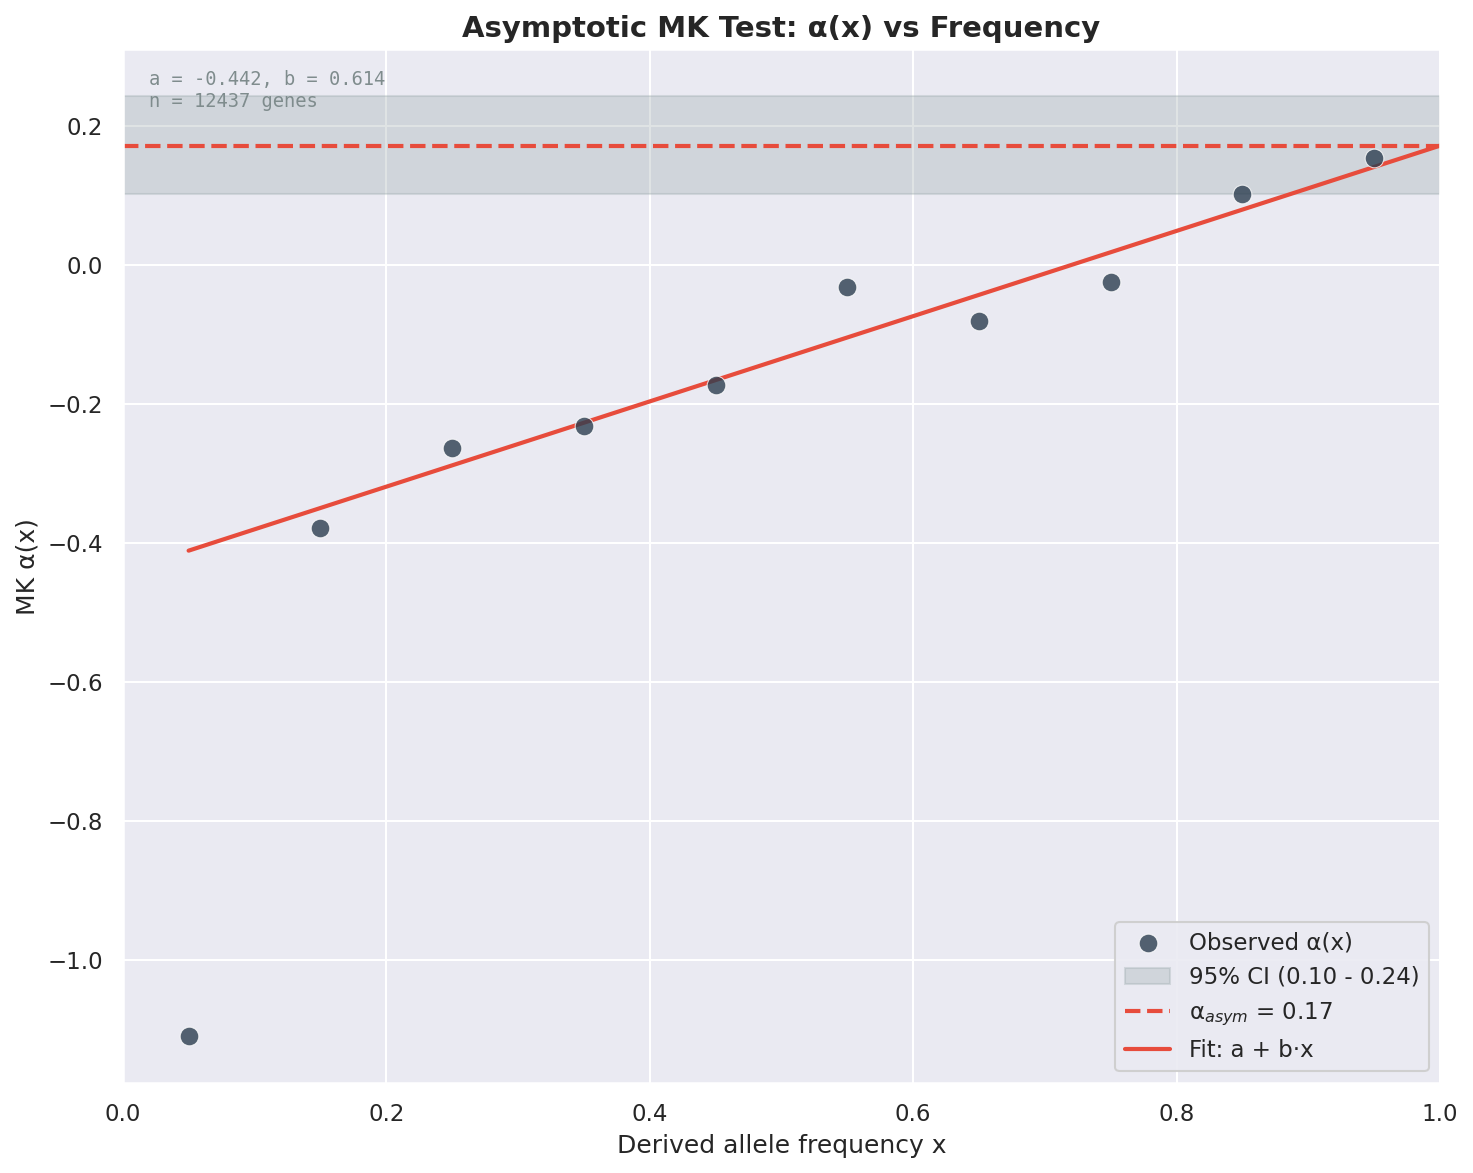
\includegraphics[width=0.48\textwidth]{figures/asymp-OH.png}
  \caption{MK test results for 12,437 human protein-coding genes using
    \textit{Pongo abelii} as the outgroup for divergence.
    % We don't have A or B in the figure above, so changing to left and right
    Left: Volcano plot from per-gene standard MK tests.
    Red points are significant after Bonferroni correction, while
    orange points are nominally significant ($p < 0.05$).
    The dashed lines indicate Bonferroni and nominal thresholds.
    The leftward shift of the cloud (NI $> 1$) reflects the
    well-known excess of weakly deleterious nonsynonymous polymorphism
    in humans.
    Right: Asymptotic $\alpha$ curve for pooled data.
    Points represent the observed $\alpha$ at each derived allele
    frequency cutoff; the solid line represents the fitted curve,
    in this case the linear model selected by AIC. The shaded area
    indicates the 95\% confidence interval around the fitted
    asymptotic $\alpha$ value.}
  \label{fig:volcano}
\end{figure*}
